\section{Turingmaschinen}

\begin{frame}[c]{Turingmaschine: Einführung}
    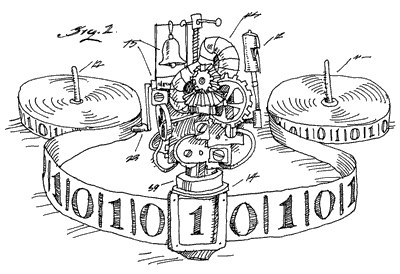
\includegraphics[width=11cm]{proseminar/images/turing-machine.png}
    % Keine Formale Definition, ist bekannt oder eben nicht
    % TM hat:
    % - Unendliches Band mit Zeichen drauf
    % - Lese & Schreibkopf
    % - State-Machine
\end{frame}


\begin{frame}[c]{Turingmaschine: Beispiel}
    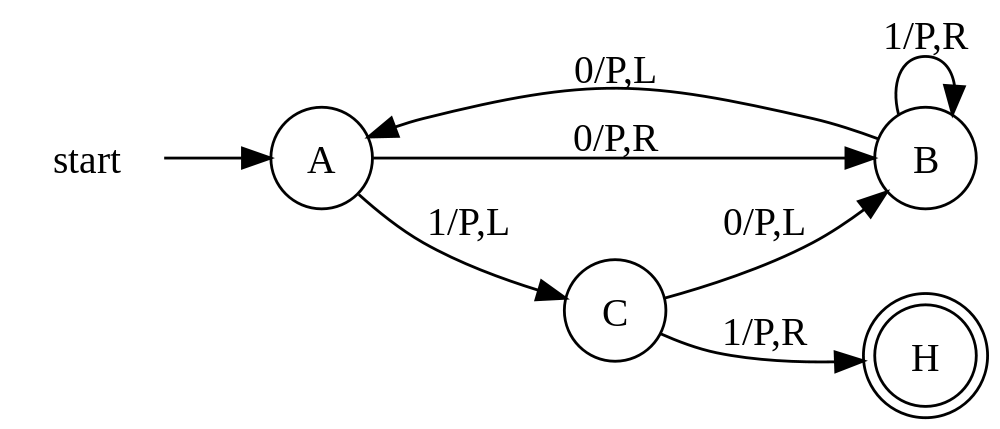
\includegraphics[width=10cm]{proseminar/images/tm-ex1.png} \\
    Schreibt 6 1er auf ein leeres Band.
\end{frame}


\begin{frame}[c]{Eigenschaften von Turingmaschinen}
    Relevant:
    \begin{itemize}
            \pause
        \item Äquivalent zu TM mit mehreren Spuren
            \pause
        \item Äquivalent zu TM mit mehreren Bändern
            \pause
        \item Beliebiges Alphabet (häufig nur Binär)
            \pause
        \item Andere Berechenbarkeitsmodelle gleichmächtig
            \pause
        \item Turingmaschine ist Codierbar
            \pause
        \item Kann andere Turingmaschinen Simulieren
            \pause
        \item Gibt abzählbar unendlich viele
%         \item Halteproblem
    \end{itemize}
\end{frame}


